\newpage
\section{Améliorations possibles}
\subsection{Maintenir une analyse constante}
Voici le scénario envisagé. L'utilisateur pose une question, le programme lui fournit une réponse. Une autre question est entrée, une nouvelle réplique est affichée. Et ainsi de suite. Pourquoi ne pas exploiter ce défilement d'informations potentiellement nouvelles ?
\subsubsection{Enregistrer les entrées de l'utilisateur}
	Supposons que le programme échoue à analyser ou à répondre à l'utilisateur. Il pourrait demander à l'utilisateur de fournir une réponse convenable à sa question, et ainsi enregistrer un nouveau couple de question réponse.

	Ou de manière bien plus transparente, il pourrait analyser la réaction de l'utilisateur suite à sa propre réponse. Il faudrait bien sûr une base de réponses désignant l'incompréhension, composée de phrases telles que "ce que tu dis n'a aucun sens" ou encore "tu racontes n'importe quoi". Si la machine reconnait une de ces phrases, elle stockerait une nouvelle association de question-réponse dans une table "à ne pas faire". Cette association doit avoir une valeur de fréquence, pour mesurer l'importance de cette réponse jugée inappropriée. En effet, certaines réponses de ce type pourraient relever du sarcasme (les smileys textuels ne sont absolument pas analysés).
\subsubsection{Suivre un fil conducteur}
	L'idée est ici de mettre en place un historique et de l'analyser pour maintenir un lien concret entre une suite de question. Il pourrait être tout à fait pertinent que le programme se concentre sur certains thèmes ou champs lexicaux de la base de données.
	Par exemple, si la conversation est particulièrement orientée "sciences appliquées", il serait intéressant de favoriser les répliques provenant d'Interstellar et autres scripts issus de films ayant ce thème.

	Concrètement, cela nécessiterait un travail de catégorisation des scripts, qui devrait se révéler relativement aisé, puisque les films sont généralement classés par genre. Mais comme les thèmes sont multiples et variés, d'autres méthodes sont certainement préférables.

\subsection{Utilisation de champs lexicaux}%Créer de nouvelles phrases, ou élargir de le champ de recherche.
	Une de ces méthodes serait l'analyse de la question non pas seulement par sa probabilité de réponse selon un corpus de texte qui va finir par devenir volumineux, mais également par le champ lexical des mots de la phrase. En effet, connaître le champ lexical des noms communs, des adjectifs ou des verbes permettrait d'élargir le champ de recherche de réponse à cette question.

	Cependant, cet élargissement du champ de recherche risquerait d'alourdir considérablement le temps de réponse, puisqu'il faudrait comparer toutes les phrases possibles pour obtenir la (ou l'une des) meilleure(s). Si ce temps d'attente reste tolérable, alors cette implémentation devrait être valide. A contrario, si la machine ne rétorque pas suffisamment vite, il faut envisager d'autres solutions.

	L'une d'entre elles serait la génération de phrases. En pratique, le champ lexical n'est pas très long à récupérer si un système performant existe déjà. Le British Lexicon Project devrait a priori pouvoir aider sur ce point. Pour générer une phrase correcte, il suffirait de voir la structure de phrase la plus fréquente (à l'aide des tags \textit{NLTK}), et de piocher dans le champ lexical des mots correspondant au type de token pour constituer une nouvelle phrase. Il s'agit bien sûr d'une méthode relativement basique ici, et d'autres plus élaborées existent certainement.

\subsection{Correction orthographique}
Une ultime amélioration apparente est celle de la correction orthographique des entrées de l'utilisateur. La manière transparente de faire serait d'accepter l'entrée de l'utilisateur, telle qu'elle est et d'y appliquer le correcteur orthographique dans l'espoir qu'il ne fasse pas d'erreur. Cette manière fonctionne particulièrement bien avec un unique (profil d') utilisateur, puisque via un processus d'apprentissage automatique, elle se familiarise avec le vocabulaire de l'individu (un des meilleurs exemples de ceci est le correcteur orthographique des smartphones).

De même, une solution valide serait de suggérer à l'utilisateur des corrections potentielles (via une interface graphique), qu'il sélectionnerait (l'illustration est ici le correcteur grammatical de Microsoft Office Word ou LibreOffice Writer).

Comment seraient suggérées ces corrections ? À l'aide d'un calcul de distance de Levenshtein, qui permet de calculer la similitude entre deux mots, en détectant les permutations, ajouts et suppressions de lettres pour arriver d'un mot à un autre. L'algorithme est relativement simple, mais s'il est appliqué à tout un dictionnaire, il risquerait d'être particulièrement gourmand en ressources. Limiter la corrections à trois ou quatre mots très proche semble raisonnable.

\section{Exemple d'exécution}

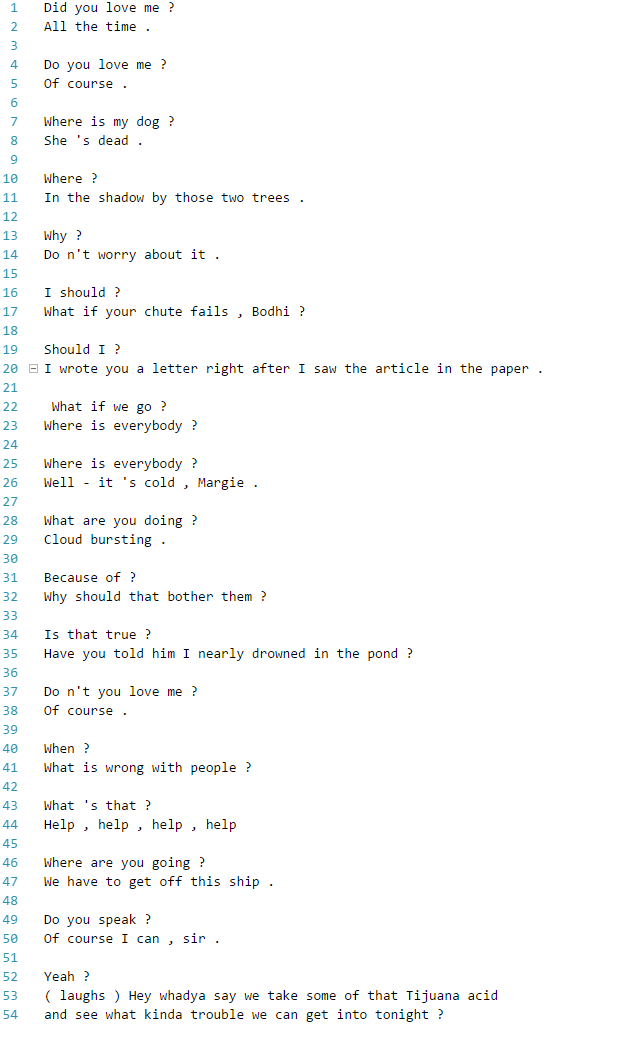
\includegraphics[scale=0.85]{executionCapture.PNG}